\section{Case Study}

\begin{frame}[plain]
	\frametitle{\polu}
	\begin{figure}
		\centering
		\begin{columns}
			\column{0.75\textwidth}
				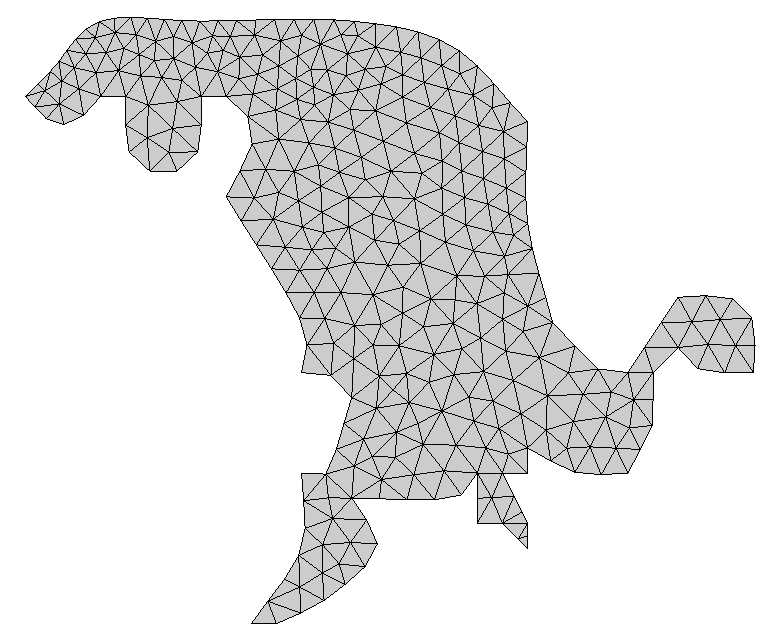
\includegraphics[width=\textwidth]{images/foz_msh.png}
				\pause

			\column{0.25\textwidth}
				\subfloat[\computeflux]{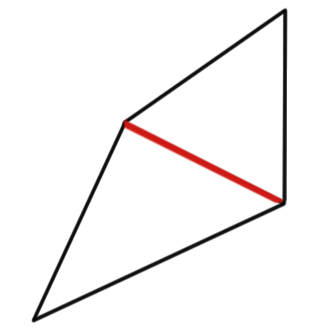
\includegraphics[width=\textwidth]{computeflux.png}}
				\vfill
				\subfloat[\update]{
\includegraphics[width=\textwidth]{update.png}}
				\vfill
		\end{columns}
	\end{figure}
\end{frame}

\begin{frame}
	\frametitle{Algorithm}

	\begin{algorithmic}
		\State $load\_input$
		\State $preprocessing$
		\While {$t \leq max_{t}$}
			\State $compute\_flux$
			\State $update$
		\EndWhile
	\end{algorithmic}
\end{frame}
